% !TEX root = main.tex
\chapter{System overview}\label{cha:systemOverview}
This chapter provides the reader with a brief overview of the whole collimator system used in the \abbrLHC at \abbrCERN as well as a more detailed description of the rotational stage, which is the device in focus in this thesis.

\section{Crystal collimators}
A collimator is a specially designed device, built to interfere with the beam and clean it from surrounding halo particles. To be able to meet the future demand of higher energy levels, a more efficient collmator is being devloped at CERN. This new collimator will utilze a crystaline solid to extract particles from the beam. The collimator consists of a T-shape structure containg two movable linear axes and one rotational stage. Each linear axis is driven by a stepping motor, labeled as \emph{M1} and \emph{M2} in Figure~\ref{fig:collimator-side}, seperately controlled in open-loop by an individual drive unit. The motor driving the vertical axis, \emph{M1}, is used to move a piece of beampipe down inside the T-shape, giving access to the horizontal axis, driven by \emph{M2}, to move the rotaional stage (including the crystal) into the beampipe to interfere with the beam. The directions of the crystal's linear and rotational movement are indicated by the arrows in Figure~\ref{fig:collimator-top}.
During operation, Physicists will drive the crystal close to the beam, enter it with an angle and rotate it slightly (in the range of \unit{10}{\milli\rad}) until the channeling effect is detected. Channeled particles will then be bent off the bem core and abosorbed further down the beam pipe.

\begin{figure}[tpb]
  \centering %crop: left bottom right top
  \subfloat[][\label{fig:collimator-side}Collimator from side]{
  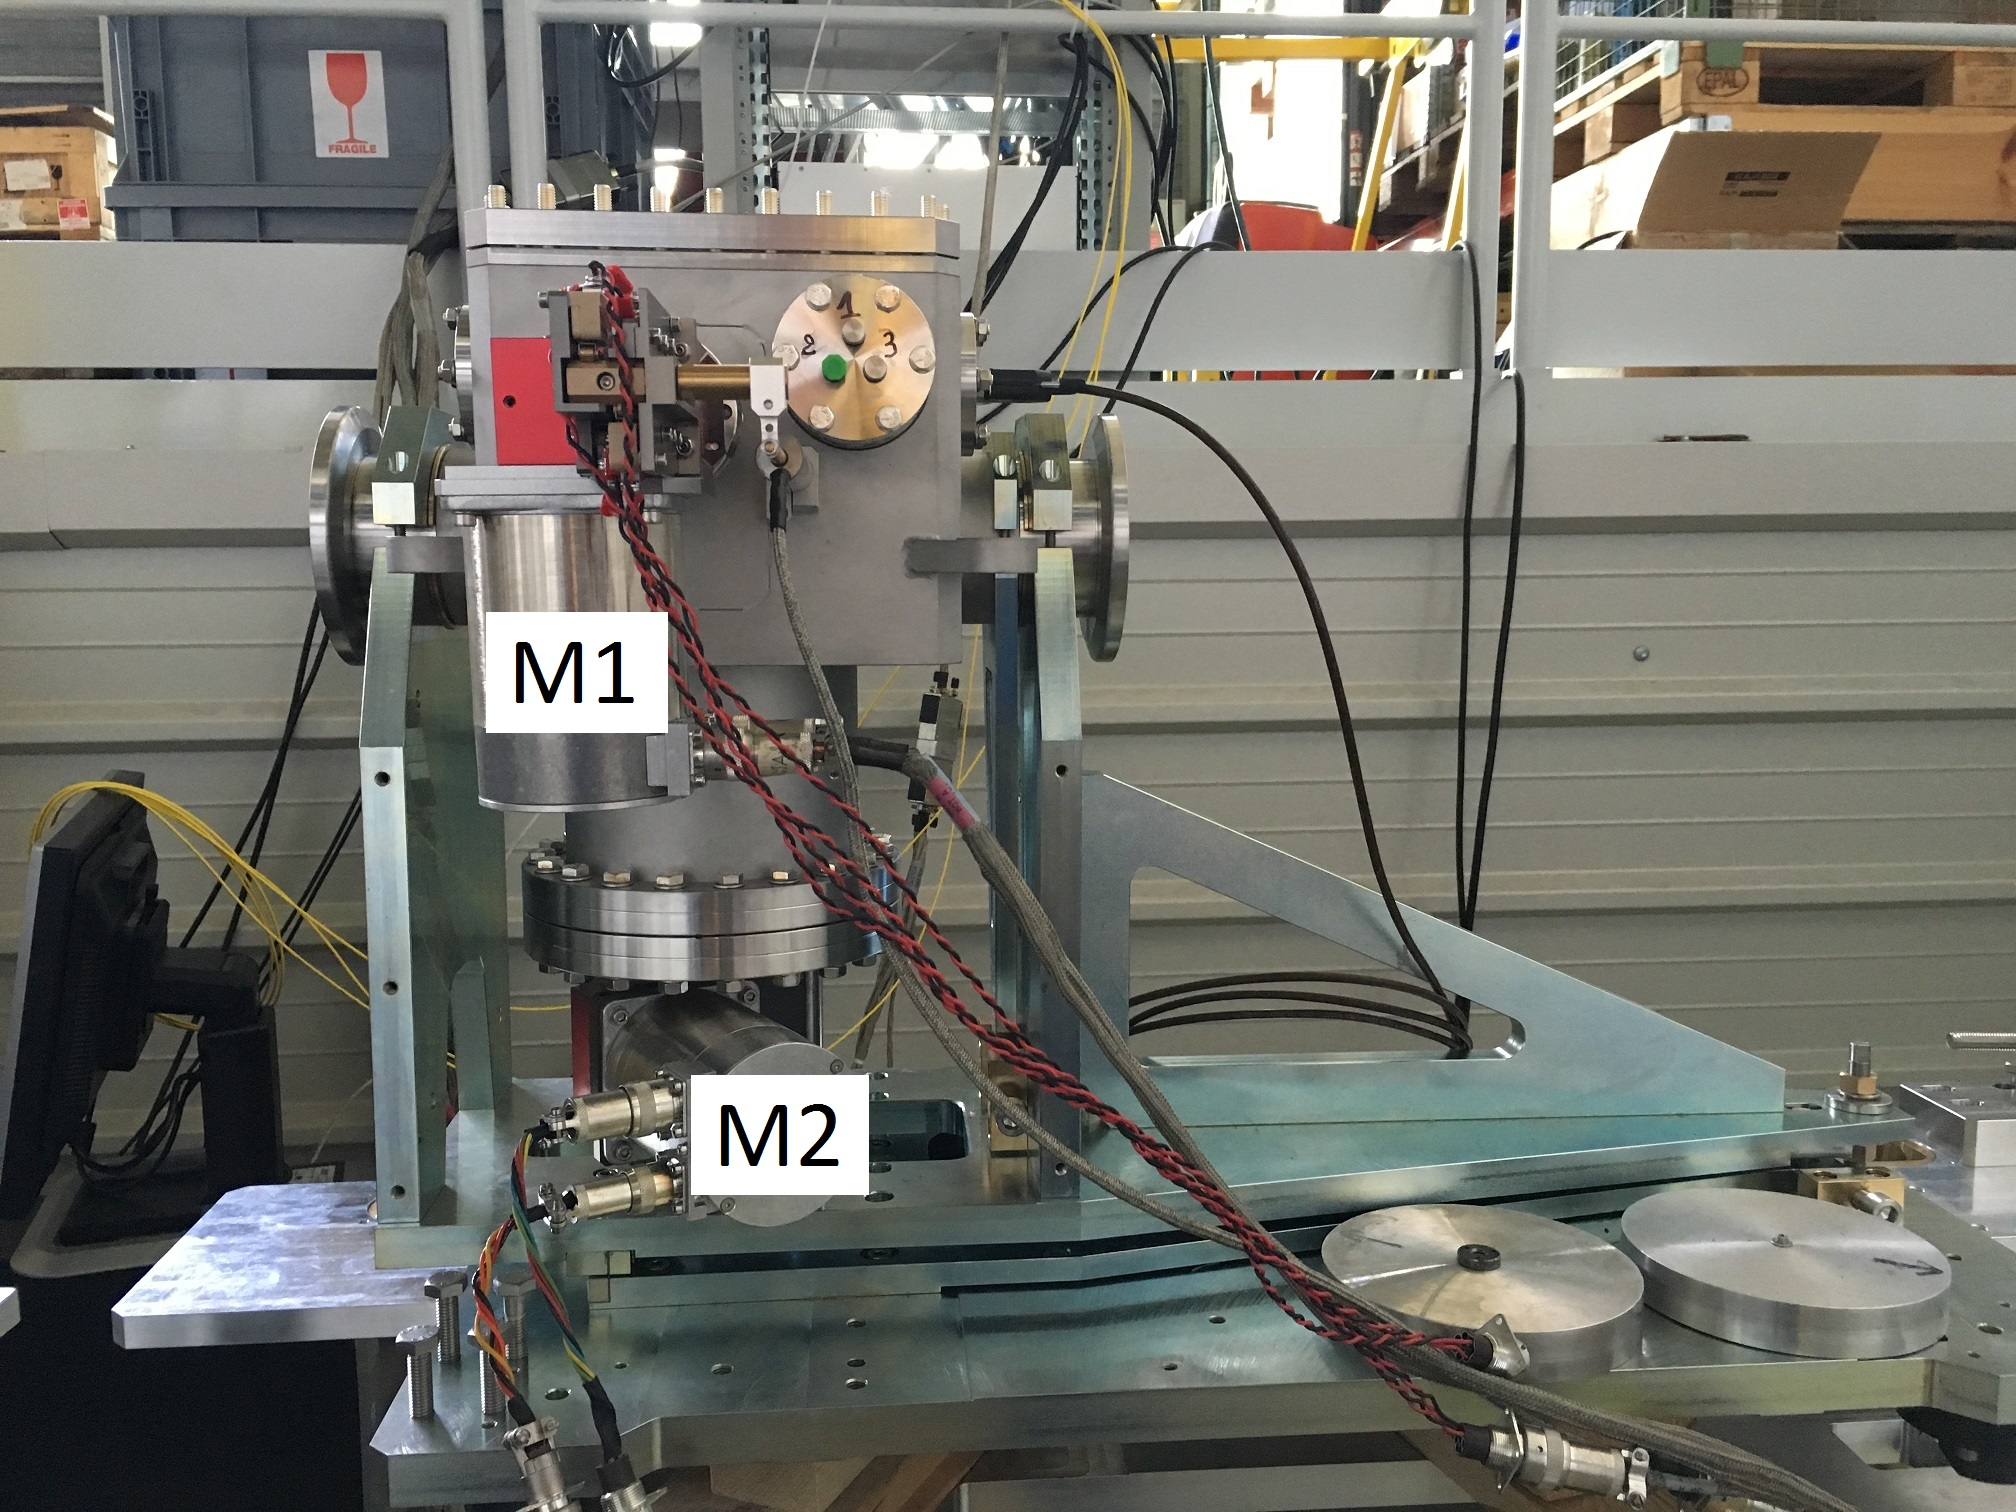
\includegraphics[width=0.5\textwidth, trim=10cm 12cm 50cm 7cm, clip=true]{fig/collimator-side}}
  \qquad
  \subfloat[][\label{fig:collimator-top}Collimator from top]{
  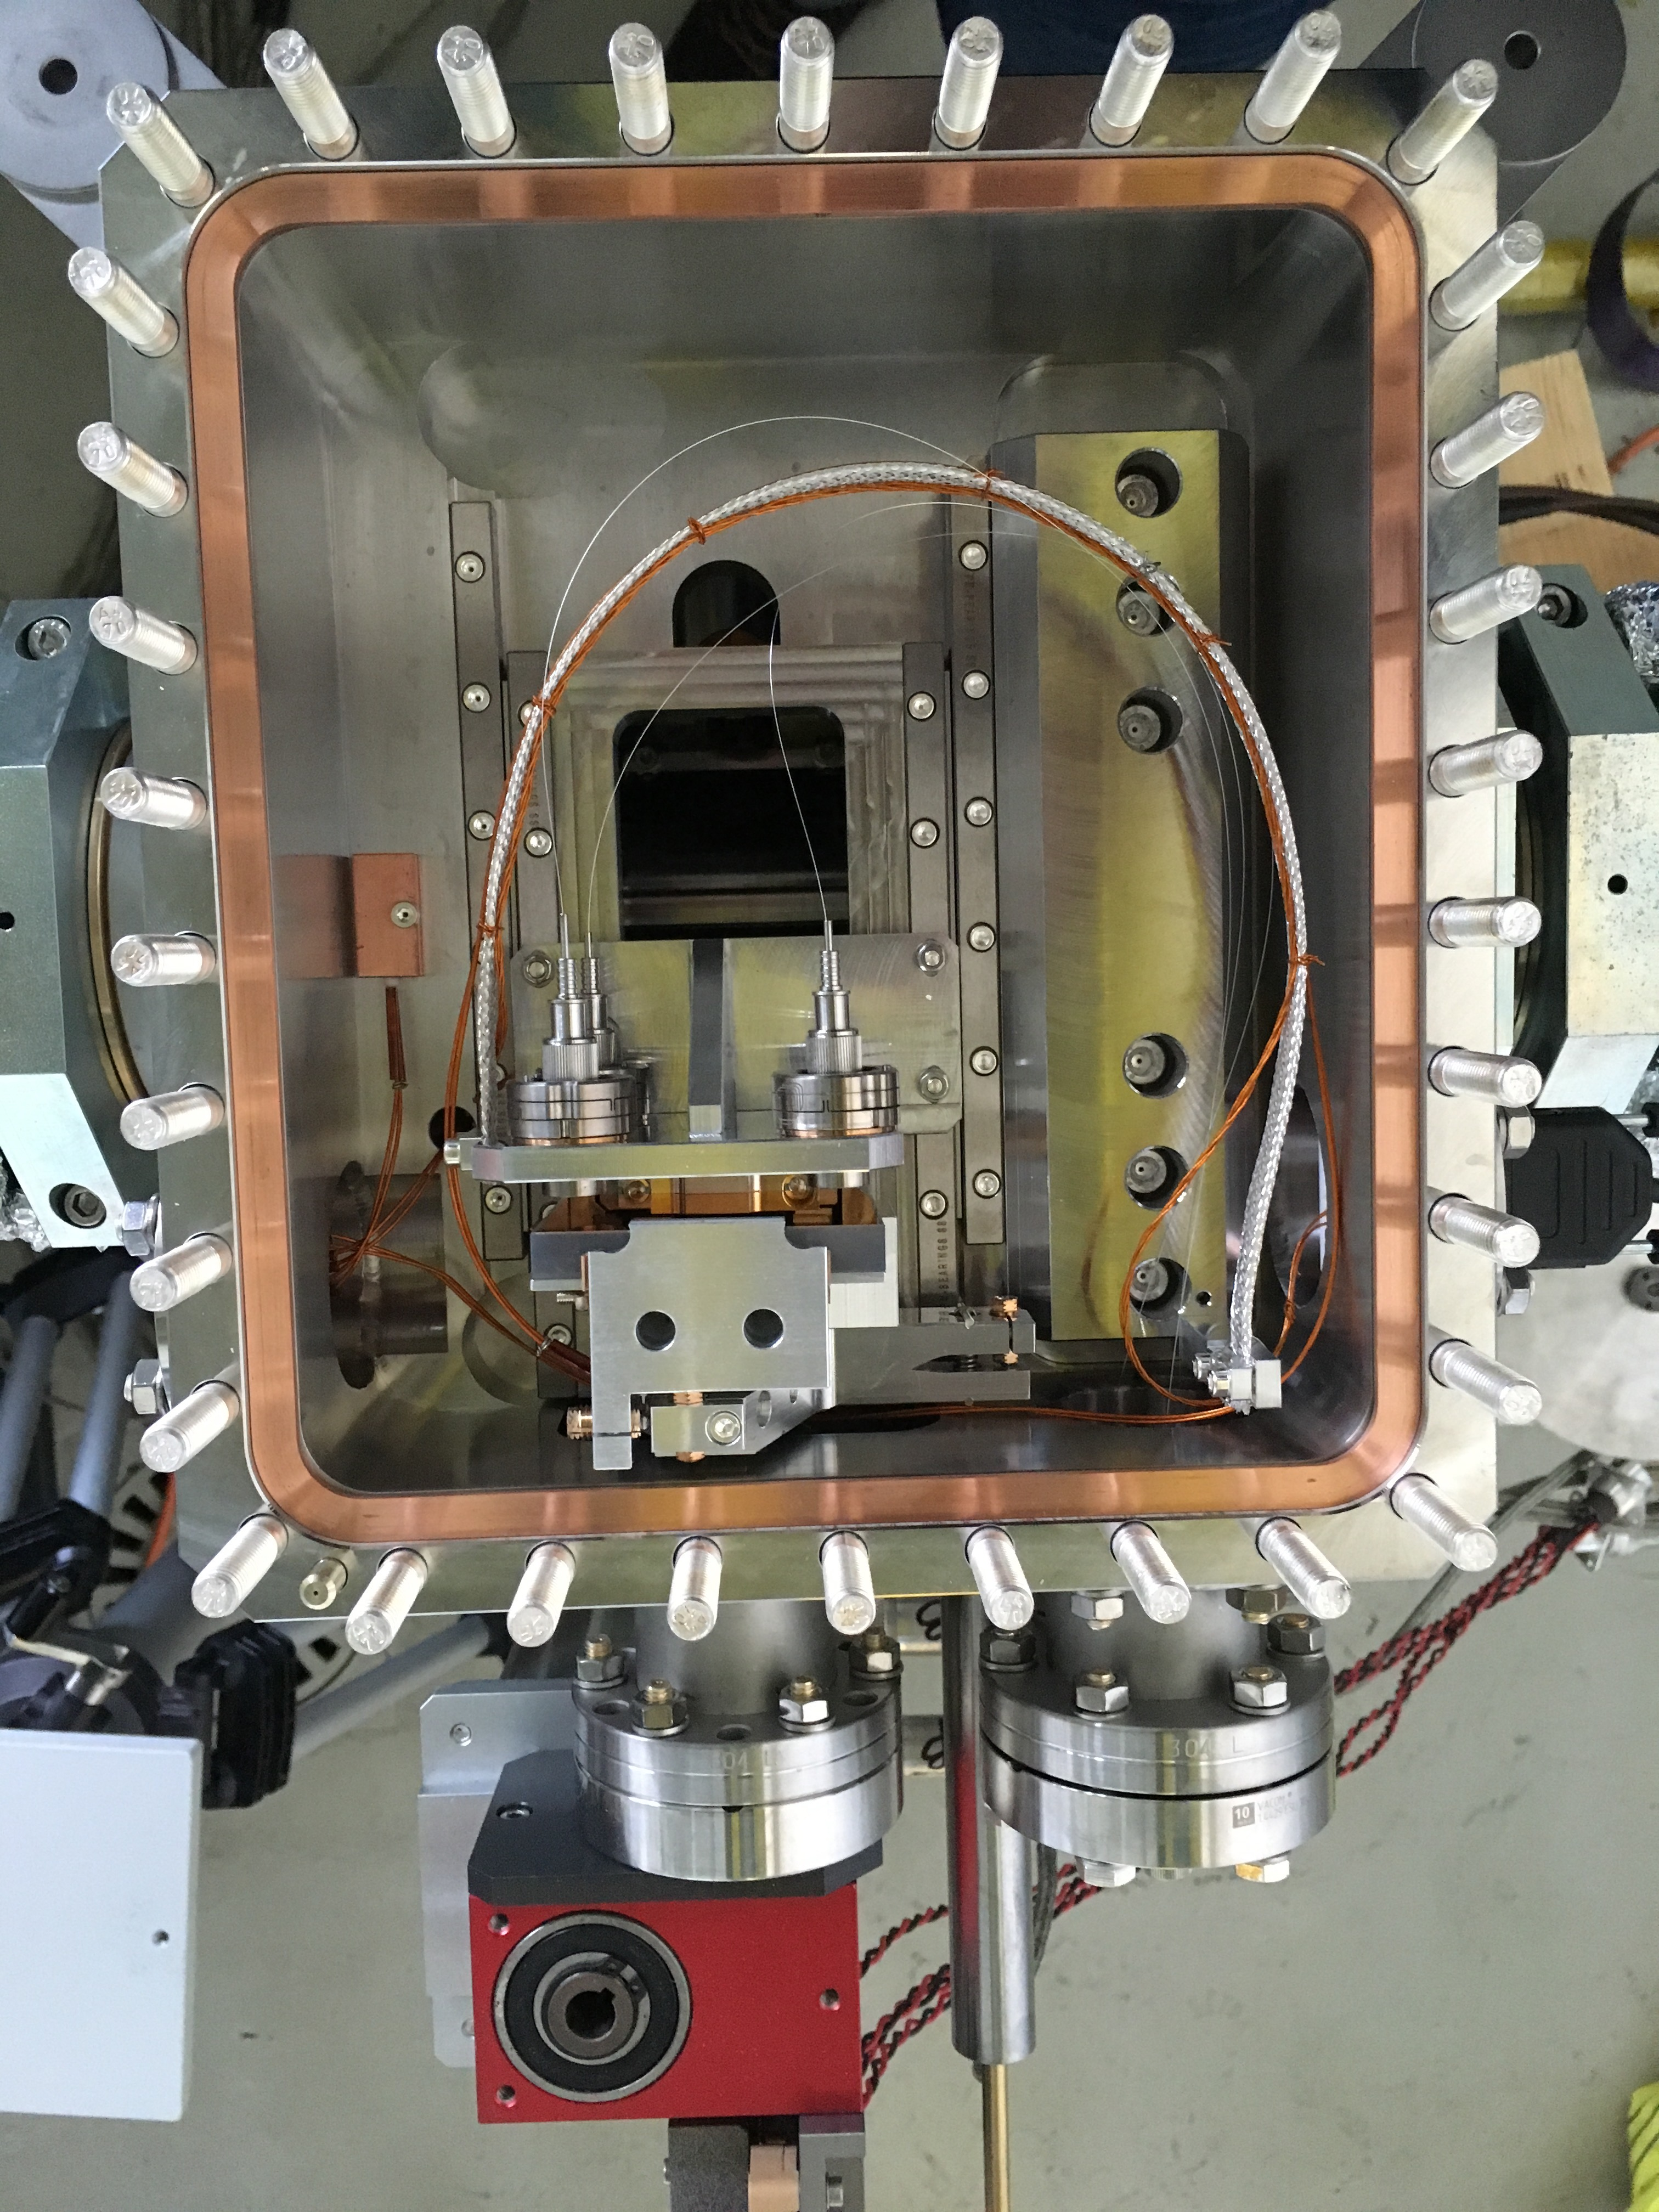
\includegraphics[width=0.4\textwidth, trim=0cm 0cm 0cm 0cm, clip=true]{fig/collimator-top}}
  \caption{\label{fig:collimator} Illustrates the collimator from the side (a) and the top (b).}
\end{figure}

\section{Rotational stage}
\label{sec:rotational_stage}
The rotational stage as shown in Figure~\ref{fig:rotationalstage}  is composed by a monolitic structure, a prestressed piezo stack actuator and an interferometer measurement system. The flexure-hinge based structure, avoids sliding parts and thereby enhance precision by reducing the number of nonlinear effects (e.g. backlash and friction). A prestressed piezo stack actuator is exploited to generate the rotaional movement by interacting on a point 4mm away from the center of rotation, see Figure.

\begin{figure}[h!]
  \centering
  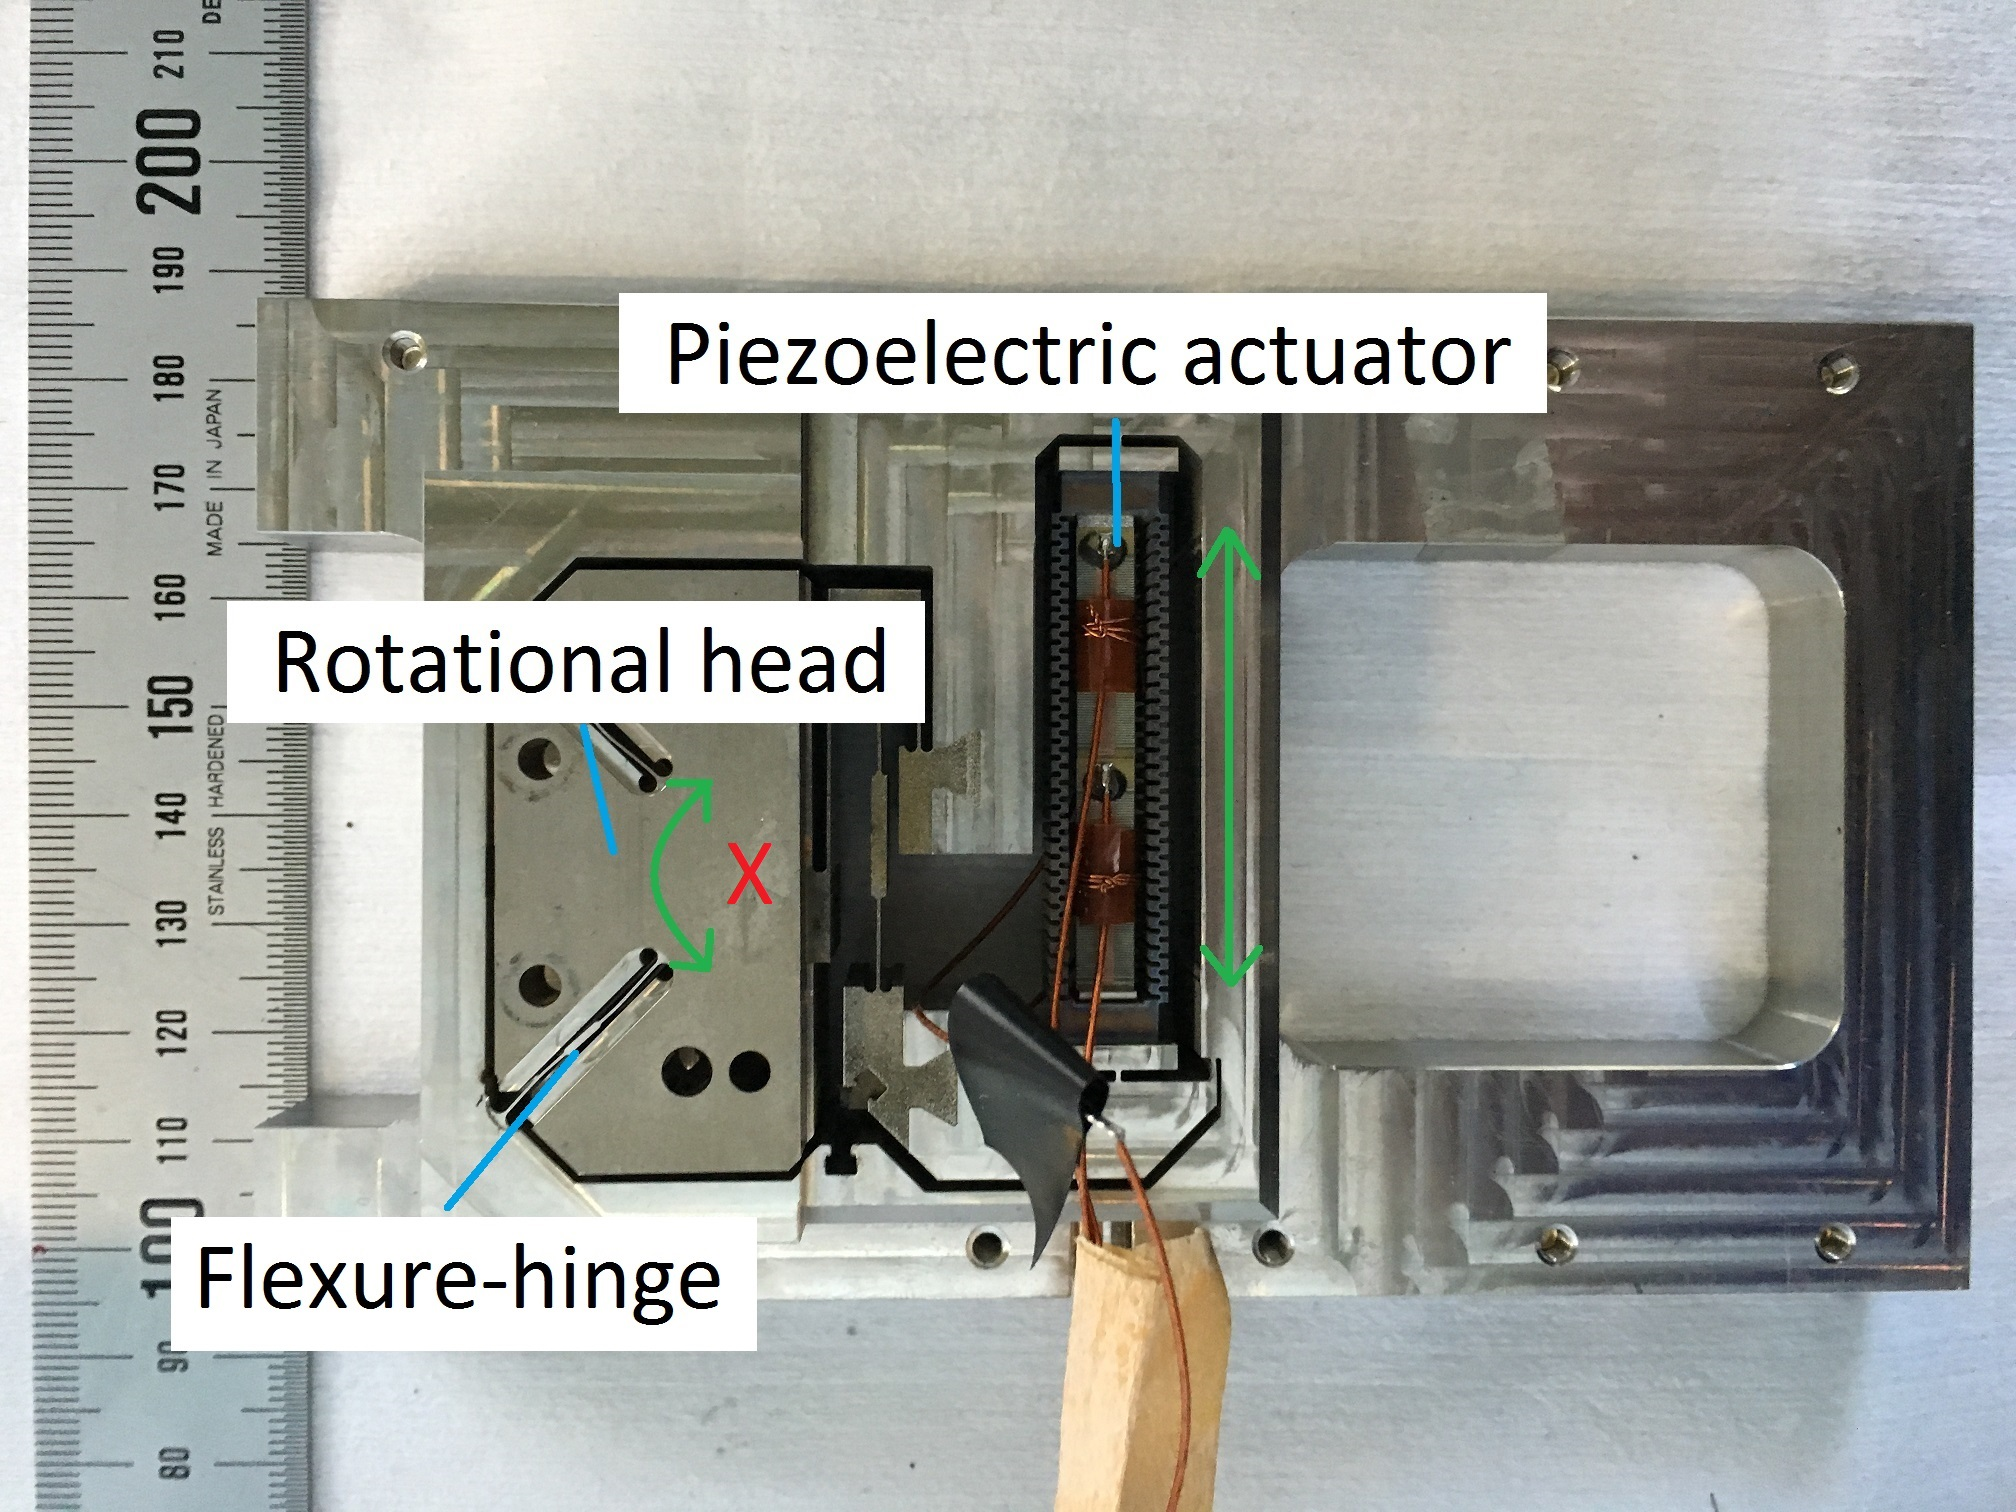
\includegraphics[width=0.5\textwidth]{fig/rotational-stage.jpg}
  \caption{\label{fig:rotationalstage} text here}
\end{figure}


This amplyfing structure gives the rotational stage a range of \unit{20}{\milli\rad}. For the measurement system, 3 interferometric heads are placed as in Figure ?, pointing towards a mirror mounted ontop of to the rotaional head, perpendicular to the plane of rotation. The setup allows for measurements of both the yaw and roll angle (the coordnate system is defined with respect to the beam). The yaw angle is used as feedback to the rotational stage control loop. The spring, depicted in Figure?, prestresses the \abbrPEA in order to enhace the overall stiffness of the stage as well as keeping the stackplates in place (the stack is nonglued to be sufficient in a radioactive area). This combinataion leads to an unmistaken resonsant structure, due to the characteristics of the \abbrPEA demanding in combination with the spring, demanding a properly designed controller. The system moving the crystal, i.e. the linear axis driven by \emph{M2} and the rotaional stage needs to be able to track reference trajectories at ramp rates of \unit{100}{\micro\radianpersecond} and reject external disturbances to maintain a maximum tracking error of $\pm$\unit{1}{\micro\rad}.

\section{Piezoelectric Stack Actuators}
The rotational stage uses a linear piezoelectric stack actuator to create the movement. It provides a displacement range from 0 to \unit{30}{\micro\meter}, corresponding to 0 and 150V, respectively. The actuators are made of many thin, stacked electroactive cheramic disks, electrically connected in parallell. This construction allows for an actuator that can exhibit the highest stiffness of all actuators designs but still with a high displacement range \cite{Piezo:2008}.

\subsection{Hysteresis Effect}
The hysteresis effect is a nonlinear effect that is present during the operation of piezopelectric actuators. It occurs when the driving direction is reversed and origins from the polarization and the molecular effects in the piezoceramic. It depends on the amplitude of the applied voltage but also on the frequency of input signals \cite{Qingson:2016}. Figure~\ref{fig:hysteresis} illustrates the hysteresis effect. One can see how the same voltage value, e.g. 60V corresponds to an angular position of \unit{5,2}{\micro\rad} in one direction and to \unit{7,2}{\micro\rad} in the opposite direction.

\begin{figure}[h]
  \centering
  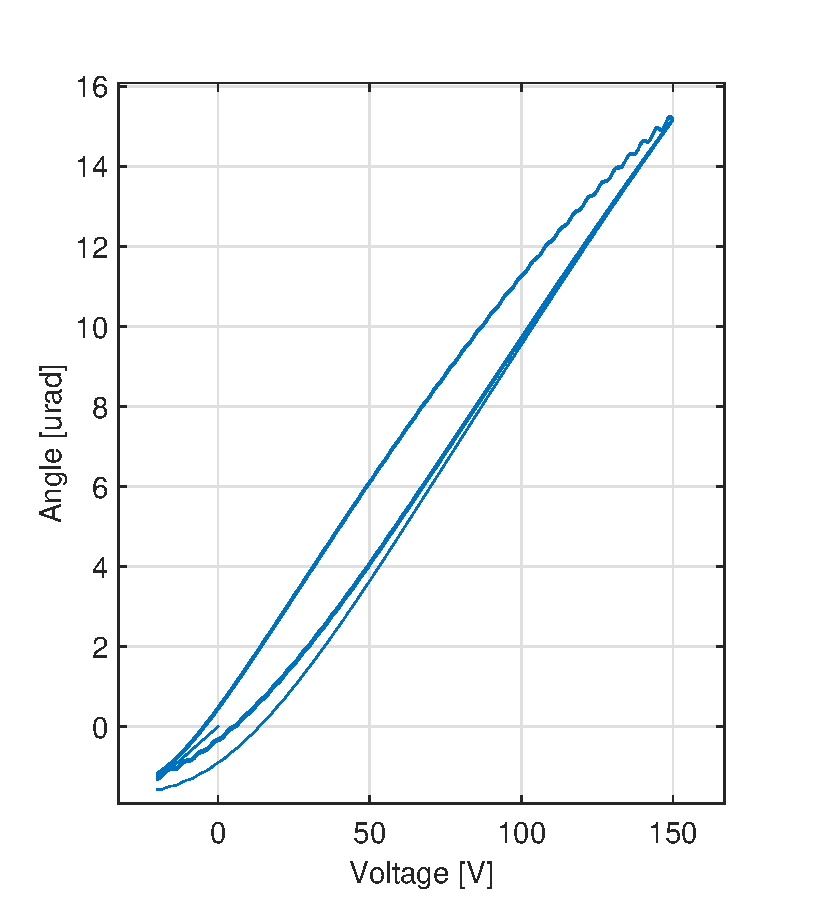
\includegraphics[width=0.5\textwidth]{fig/matlab/hysteresis.eps}
  \caption{\label{fig:hysteresis}Illustration of the hysteresis effect.}
\end{figure}

\subsection{Creep Effect}
The creep effect is another nonlinear effect that is present during the operation of piezoelectric actuators. The effect is a slow elongation or contraction of the actuator displacement over time, with a constant driving signal and is caused by thermal effects in the piezoceramics. Figure~\ref{fig:creep} illustrates the creep effect. One can see how the rotational stage slightly drifts in rotation after the applied negative step.

\begin{figure}[h]
  \centering
  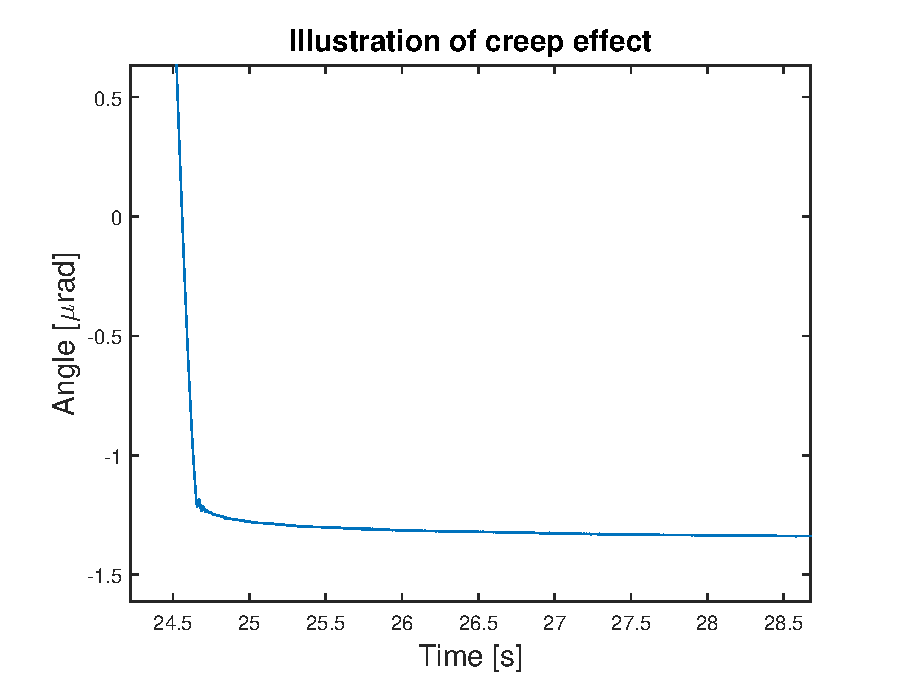
\includegraphics[width=0.5\textwidth]{fig/matlab/creep.eps}
  \caption{\label{fig:creep}Illustration of the creep effect. Note that the creep effect can last up to 10-15 minutes even if the plot only shows the development over 4 seconds.}
\end{figure}

The creep effect is in this project (and many others) effeciently suppressed by the feedback controller requiring no precise modeling and cancellation techniques.

\section{Rotational Stage Modeling}
The piezoactuated rotational stage is modelled by a Hammerstein structure, adopted by the authors in \cite{ButcherController:2015}, allowing them in principal, to decouple the nonlinear hysteresis from the linear system dynamics. The employed Hammerstein structure is depicted in Figure~\ref{fig:hammerstein} and consists of a \emph{Static Hysteresis} (rate independent) model and a \emph{Linear Dynamics} model. {\abbrPEA}s are known to show hysteretic behavior with a nonlocal memory (the current output does not only depend on the current input voltage but also on its history) as described in \cite{ButcherIdentification:2015}. This behvaiour is modeled by a generalised Maxwell-slip compensation model, described in \ref{sec:maxwell}. The extracted linear dynamics is identified using the described procedure in \ref{sec:linsys}

\begin{figure}[h]
  \centering %crop: left bottom right top
  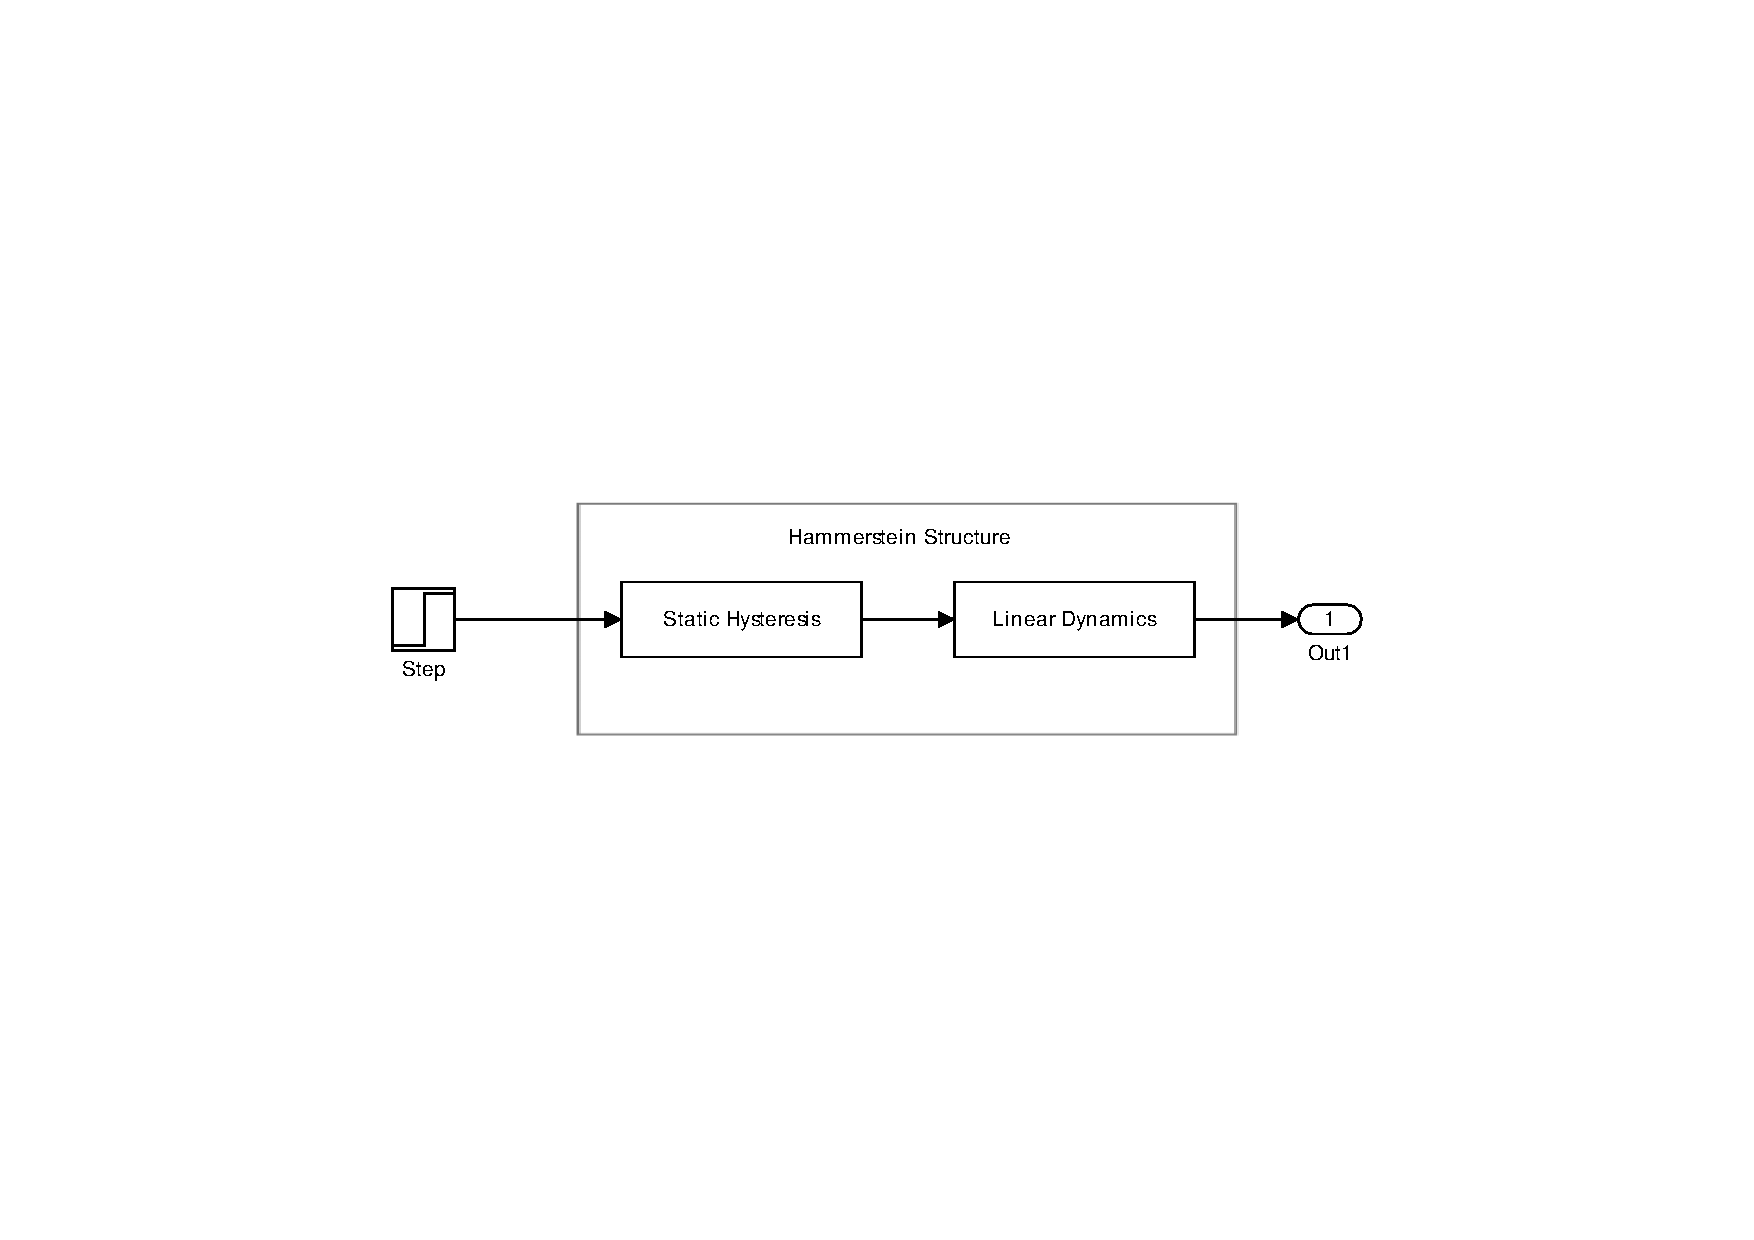
\includegraphics[width=0.7\textwidth, trim=8cm 8cm 7.73cm 8cm, clip=true]{fig/matlab/hammerstein}
  \caption{\label{fig:hammerstein}Block diagram of the Hammerstein structure, consisting of two blocks in series, modeling the static hysteresis and the linear dynanamics, respectively.}
\end{figure}

\subsection{Maxwell-slip Model}
\label{sec:maxwell}
A generalized Maxwell-slip is used to model the hysteresis effect. It uses a parallell $n^{th}$ order elasto-slide element system with a friction force acting on each element, to create a nonlinear model. An elasto-slide element consist of a massless spring connected in series with a massless block that is subject to Coulomb friction. The model is summerized in the following equations and described more thourghly in \citep{Ru:2016}.

\begin{equation}
  \label{eq:maxwell_slip}
  F_i =
  \begin{cases}
    k_i(x - x_{bi}) & \quad \text{if }  k_i|x - x_{bi}| < f_i\\
    f_isgn(\dot{x}) \text{ and } x_{bi} = x - \frac{f_i}{k_i}sgn(\dot{x})  & \quad \text{else}\\
  \end{cases}
\end{equation}

\begin{equation}
  \label{eq:maxwell_sum}
  F = \displaystyle\sum_{i=1}^{n} F_i
\end{equation}

Where $F_i$ is (in terms of the rotational stage) the applied voltage, $x$ the rotaional displacement, $x_b$ blocked displacement and $k_i, f_i$ are unkown parameters where $i=1 \hdots n$ . The model parameters have been estimated by fitting the model to the major hysteresis loop, obtained by acquiring data from the system with a 0.5 Hz input driving signal as described in \cite{ButcherIdentification:2015,ButcherController:2015}. The result is presented in Figure~\ref{fig:maxwell} and Table~\ref{tab:maxwell} where $n=10$.

\begin{figure}[h]
  \centering
  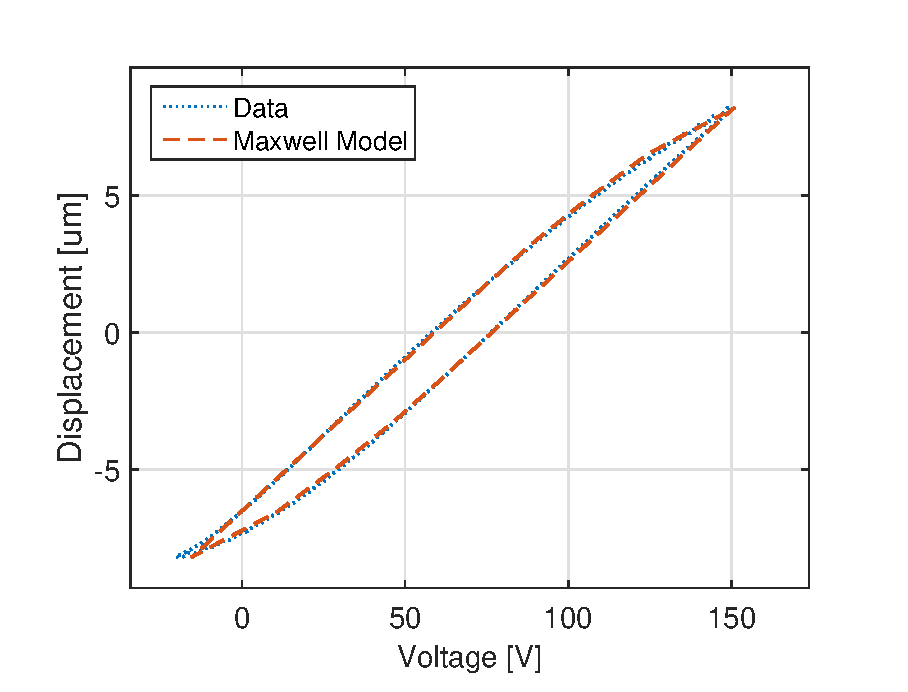
\includegraphics[width=0.5\textwidth]{fig/matlab/maxwell.eps}
  \caption{\label{fig:maxwell} The plot shows the model fit of the Maxwell slip model to the acquired hysteresis of the rotational stage. The fit has a mean squared error of 1.1464.}
\end{figure}

\begin{table}[h!]
  \centering
  \begin{tabular}{| l | l | l |}
    \hline
    $i$ & $k_i$ & $f_i$ \\ \hline
    1 & 4.53 & 3.69 \\
    2 & 0.90 & 1.46 \\
    3 & 1.01 & 2.47 \\
    4 & 0.36 & 1.16 \\
    5 & $1.49 \times 10^{-6}$ & $4.28 \times 10^{-6}$ \\
    6 & $2.89 \times 10^{-7}$ & $1.41 \times 10^{-6}$ \\
    7 & $1.59 \times 10^{-7}$ & $9.10 \times 10^{-7}$ \\
    8 & $1.39 \times 10^{-7}$ & $9.10 \times 10^{-7}$ \\
    9 & $2.28 \times 10^{-7}$ & $1.67 \times 10^{-6}$ \\
    10 & $4.58$ & 37.30 \\
    \hline
  \end{tabular}
  \caption{\label{tab:maxwell} Identified parameters of the Maxwell slip model.}
\end{table}

\subsection{Linear System Identification}
\label{sec:linsys}
The extracted linear dynamics has been identified as an $6^{th}$ order Output-Error system using a \abbrPRBS as excitation signal, allowing for a valid extraction from the nonlinear dynamics. The system transfer function has been derived in discrete-time using the the System Identification Toolbox in Matlab. A more detail description of the procedure is available in \citep{ButcherController:2015}. Figure~\ref{fig:model} shows a comparison between the model and the real system in the frequency domain, where the Fast Fourier Transform (\abbrFFT) identification is calculated by dividing the \abbrFFT of the output with the \abbrFFT of the input.

 The transfer function of the model, discretized with a sampling time of \unit{0.5}{\milli\second}, is presented in \eqref{eq:tf}.

\begin{equation}
  \label{eq:tf}
  G_o(z) = \frac{21.05z^{-1} - 6.85z^{-2} + 8.52z^{-3} - 0.71z^{-4} + 9.30z^{-5}}{1 - 1.85z^{-1} + 1.09z^{-2} + 0.016z^{-3} - 1.32z^{-4} + 1.55z^{-5} - 0.48z^{-6}}
\end{equation}

\begin{figure}[h]
  \centering
  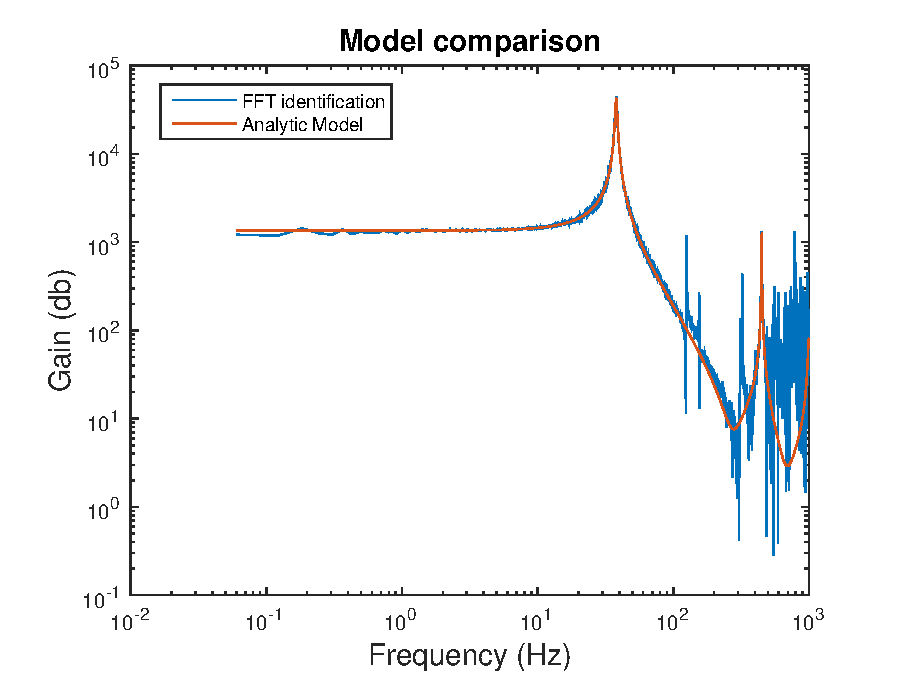
\includegraphics[width=0.5\textwidth]{fig/matlab/model.eps}
  \caption{\label{fig:model} The plot shows the model fit of the Maxwell slip model to the acquired hysteresis of the rotational stage. The fit has a mean squared error of 1.1464.}
\end{figure}

\section{Present Control Approach}
The original controller for the rotational stage is a 2-\abbrDOF structure (feedback and pre-filter). A schematic overview of the control loop is depicted in Figure~\ref{fig:present}, consisting of a controller block C, a prefilter F, a disturbance d and the linearized rotational stage $G =G_oH^{-1}$, where $G_o$, $H^{-1}$ is the linear dynamics and the hysteresis compensator, respectively.

\begin{figure}[h]
  \centering %crop: left bottom right top
  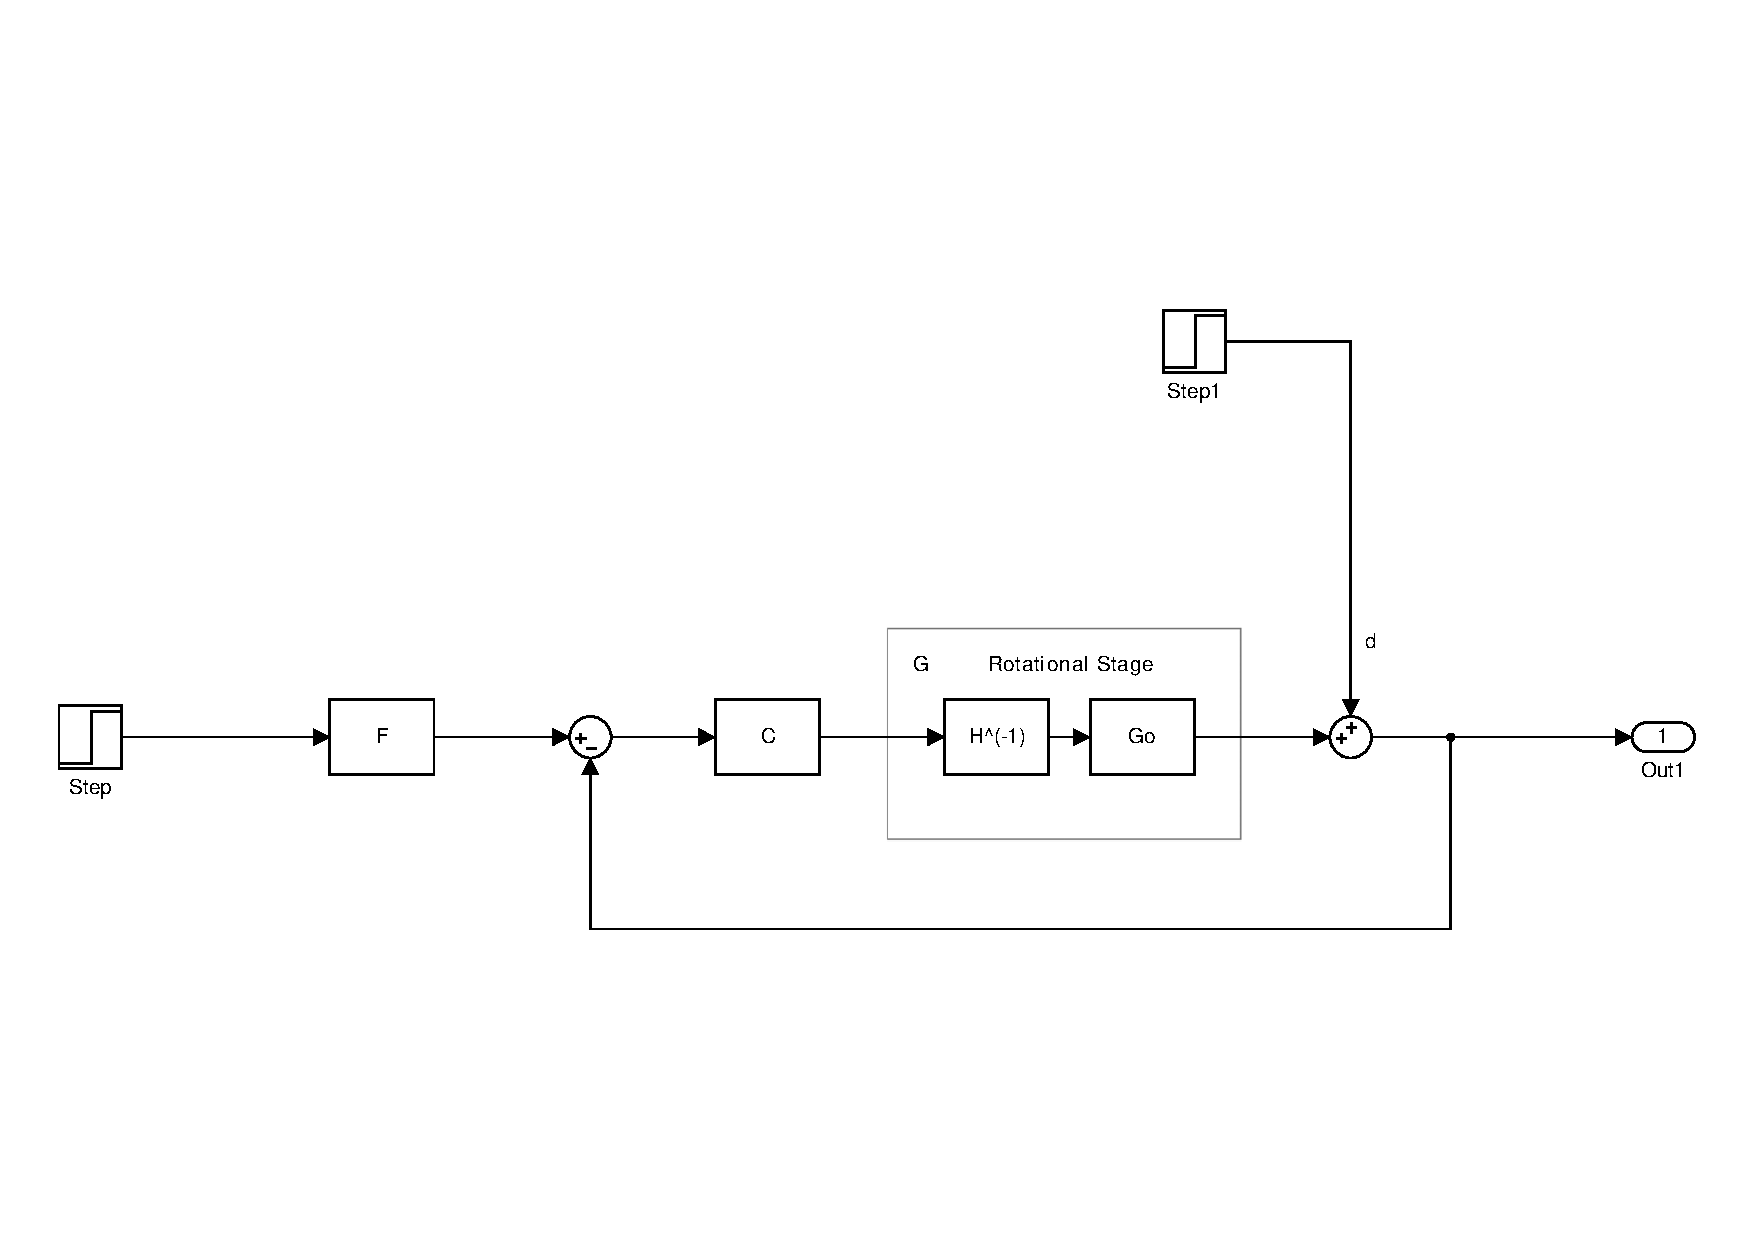
\includegraphics[width=1\textwidth, trim=4cm 3cm 2.1cm 10cm, clip=true]{fig/matlab/present_controller}
  \caption{\label{fig:present}Block diagram of the present control loop, inlcuding controller, prefilter and hysteresis compensator.}
\end{figure}

The controller block (C) is a series combination of a \abbrPID controller, notch filter and a lead network, aiming to stabilize the system (\abbrPID), increase the sufficient phase margin (lead) and make the system robust to high frequency oscillations (notch). Since the bandwidth of the system is relatively low, $f_b = 58 Hz$ according to  Figure~\ref{fig:model}, it has been decided to exclude cancellation of the first resonance peak in order to keep the bandwith as high as possible and have a sufficient attenuation on the sensitivity function \citep{ButcherController:2015}. The PID controller, lead network and notch filter are all presented below in \eqref{eq:controller}.

\begin{subequations}
  \label{eq:controller}
\begin{alignat}{2}
  \label{eq:pre}
  & F = \frac{0.0029z - 0.0029}{z^3 - 2.91z^2 + 2.816 z - 0.91} \\
  \label{eq:pid}
  & C_{PID} = \frac{0.47z^2 - 0.94z + 0.47}{z^2 - 1.78 z + 0.78} \\
  \label{eq:lead}
  & C_{lead} = \frac{4.20 z^2 - 7.72z + 3.55}{z^2 - 1.67z + 0.69} \\
  \label{eq:notch}
  & C_{notch} = \frac{0.28z^4 - 0.62z^3 + 0.75z^2 - 0.59z + 0.26}{z^4 - 1.95z^3 + 1.39z^2 - 0.40z + 0.039}
\end{alignat}
\end{subequations}
